\documentclass[12pt,a4paper]{ctexart}
\usepackage{ctex}
\usepackage{emptypage} 
\usepackage{fancyhdr}
\usepackage{amsmath,amsfonts,amssymb,mathtools}
\usepackage{graphicx}
\usepackage{mathptmx}
\usepackage{booktabs}
\usepackage[labelfont=bf]{caption}
\usepackage{indentfirst}
\usepackage{caption}
\usepackage{enumitem}
\usepackage[marginal]{footmisc}
\usepackage{subfigure}
\usepackage{fontspec}
\usepackage{geometry}
\usepackage{setspace}
\usepackage{listings}
\usepackage{xcolor}
\usepackage{float}
\newgeometry{left=3cm,top=2.5cm,bottom=2.5cm,right=3cm}
\setmainfont{Times New Roman}
\setCJKmainfont[BoldFont=SimHei,ItalicFont=KaiTi]{SimSun}

\lstset{
	backgroundcolor=\color{green!10!blue!15},
	rulesepcolor= \color{red!40!blue!100},
	breaklines=true,
	breakatwhitespace=false,
	numbers=left, 
	numberstyle= \small,
	keywordstyle= \color{blue},
	commentstyle=\color{gray}, 
	frame=shadowbox
}

\renewcommand{\baselinestretch}{1.5}

\title{\textbf{浅析歌声合成技术的发展史}}

\author{
\\
\Large{麻超 \quad 201300066}
\\[6pt]
{ \large \textit{南京大学人工智能学院}}\\[2pt]\large \textit{maple@smail.nju.edu.cn}
}

\date{}
\newcommand{\supercite}[1]{\textsuperscript{\cite{#1}}}

\begin{document}
\maketitle
\setcounter{page}{1}
\textbf{摘要} \quad {1961年,歌声合成第一次出现在大众面前,而在近年来的发展过程中,其技术经历了几次迭代,从最早的波形拼接法,我们需要将每个音符和其任意两者之间的转折都穷举出来,并拼接得到完整的歌声。随后,又出现了数学建模方法进行歌声合成,我们可以利用声码器对声音进行分析,并利用频谱包络方法得到更好的歌声。但随着数学建模方法触碰到瓶颈,我们需要用更合适的方法,如机器学习,对歌声进行更高效、更逼真的合成,助力技术发展。} \\

\textbf{关键词}\quad {声音合成,声码器,机器学习,频谱包络}
\\[60pt]
\section{引言}
1961 年,贝尔实验室的研究人员在使用 IBM7094 超级计算机研究语音合成时,决定尝试一下合成歌声。John Kelly 和 Carol Lockbaum 负责了人声生成部分,Max Mathews 负责了伴奏生成。他们选择了《Daisy Bell》这首当时已相当知名的爱情歌曲。《Daisy Bell》因此成为了世界上第一首由计算机合成人声演唱的歌曲\supercite{1}。近年来,人工智能技术飞速发展,在声音合成领域取得了非常显著的成绩,也有着非常多的应用,无论是AI配音,以洛天依为代表的虚拟歌手,或者是还原人的声音,成果都非常多。现在流行的“营销号解说”,大多数都是利用了人工智能技术的配音,而从十多年前开始,初音未来、洛天依、乐正绫等一系列虚拟歌手引得人们注意,到现在,他们的技术飞速发展,已经成为了许多晚会不可或缺的项目,其他方面,我们还可用声音合成完成许多过去难以完成的事情,比如在《流浪地球2》电影预告片里就提到了李雪健老师的声音是由AI合成完成的\supercite{2}。本文将简单介绍歌声合成的几个阶段和主要方法。

\section{源·滤波器模型}
人类发音系统由独立的两部分组成,即源·滤波器模型,这一观点是1942年由千叶和梶山在其著作《The Vowel: Its nature and structure》(元音的性质与结构)中首次提出并一直沿用至今。该模型认为人类发音系统由独立的两部分组成,其中声带作为源振动发声,发出的信号经过一个由声道、喉咙、口腔、鼻腔、牙齿与嘴唇构成的滤波器系统拥有了特定的频谱。源决定了声音信号的频率。在讲话时,肺部挤出空气产生气流。当声带收缩闭合时,气流冲激冲击声带产生有规律振动,发出周期性的气流脉冲\supercite{3}。单个脉冲的数学表达式近似如下所示:
\begin{equation}
    g(n)=
    \begin{cases}
        \frac{1}{2}[1-\cos(\pi n/N_1)], & 0\leq n\leq N_1 \\
        \cos [\pi(n-N_2)/2N_2],         & N_1<n<N_1+N_2   \\
        0,                              & else
    \end{cases}
\end{equation}

其中$N_1$为上升时间,$N_2$为下降时间\supercite{4}。

脉冲的频率即为人声的基频。声带的发生的频率同时受声带的物理性质和紧张程度来控制。滤波器的性质决定了声音的频谱(spectrogram),频谱则决定的声音的音色和表达的内容。源发出的脉冲在经过滤波器系统后,其谐波会被不同程度的增强和减弱。频谱上谐波能量强的区域被称为共振峰。这些语音按一定节奏和频率规律发出,就有了歌声。理论上,只要知道每个音的频谱特征和基频,就可以通过逆变换得到波形。
\section{波形拼接法}
人在说话和歌唱时,每个字每个词都包含数个元音辅音。共鸣腔的频率响应也不断变换着,频谱是动态的,让语言信号处理变复杂了很多。考虑到这些因素,基于源 - 滤波器的人声合成需要复杂的算法和较高的处理器性能,否则听起来很假。因此早期合成软件纷纷采用了一种取巧的方案:波形拼接。

简单来说,波形拼接的语音合成提前录制好各种基本语素的采样,在使用的时候将波形升降调到需要的音高,再组成句子。语音合成软件多数使用国际音标(International Phonetic Alphabet,IPA)来标记发音。原版 IPA 包含较多的特殊字符,为了方便计算机输入,常使用 X-SAMPA 等记法。最知名的波形拼接语音合成软件可能是雅马哈的 VOCALOID。以 VOCALOID4 为例,其.ddb 声库文件中包含了一系列预先录制好的元音,辅音,以及音与音之间衔接的采样。如下图所示:
\begin{figure}[H]
    \centering
    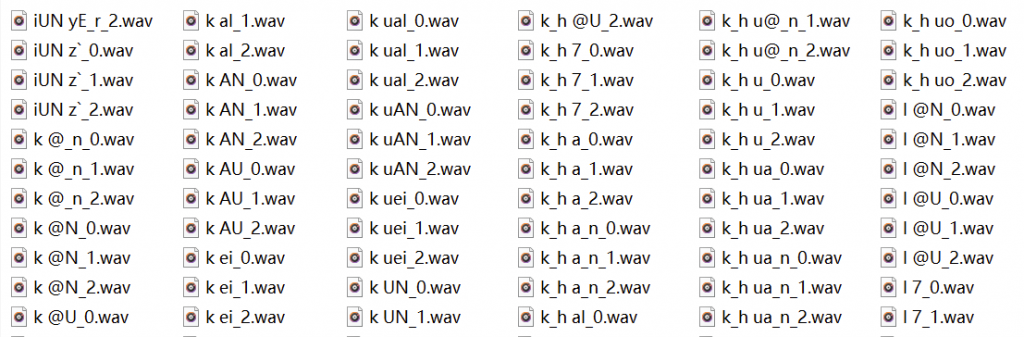
\includegraphics[height=4.5cm]{figure1.png}
    \caption{VOCALOID4采样库}
\end{figure}
其总采样数大约7600个。数量如此之多的原因是波形拼接算法很难处理好音与音之间的过渡,所以只能把所有过渡都枚举式的录制出来。考虑到唱高音和唱低音时的音色变换,声库中每个音素都分三个音高录制了三份。合成语音时,编辑器从声库中自动选择需要的音素拼在一起。波形拼接法对音色保留较好,对性能要求低,但它的缺陷也很明显。波形拼接法在制作声库时需要录制大量(数千)的声音样本并进行人工标注,费时费力。山新本人曾吐槽过洛天依音源 “录音表特别长”。此外,由于同音素使用的是重复的采样,音色不能根据音高、情感、音量、速度来变化,真实度存在瓶颈。如今波形拼接法正在被逐渐弃用,雅马哈的 VOCALOID5 是最后一代使用此方法的歌声合成引擎\supercite{5}。从VOCALOID6开始,其将新增基于深度神经网络的Vocaloid:AI引擎。

\section{统计模型与声码器法}
声码器(Vocodor)可以将语音信号转换为一系列参数或将参数转换回语音信号。1938 年,贝尔实验室的 Homer Dudley 发明了第一台能够解码和合成人声的声码器装置。声码器最初用于通信传输中的加密和节省带宽,后来也用于电子音乐的制作中。著名电子乐队蠢朋克(Daft Punk)歌曲中的” 机器人” 人声就是用声码器制作的。声码器的原理是人声的源 - 滤波器模型。声码器利用 STFT 短时傅里叶变换将语音分片,并取得其频率分布\supercite{6}:
\begin{figure}[H]
    \centering
    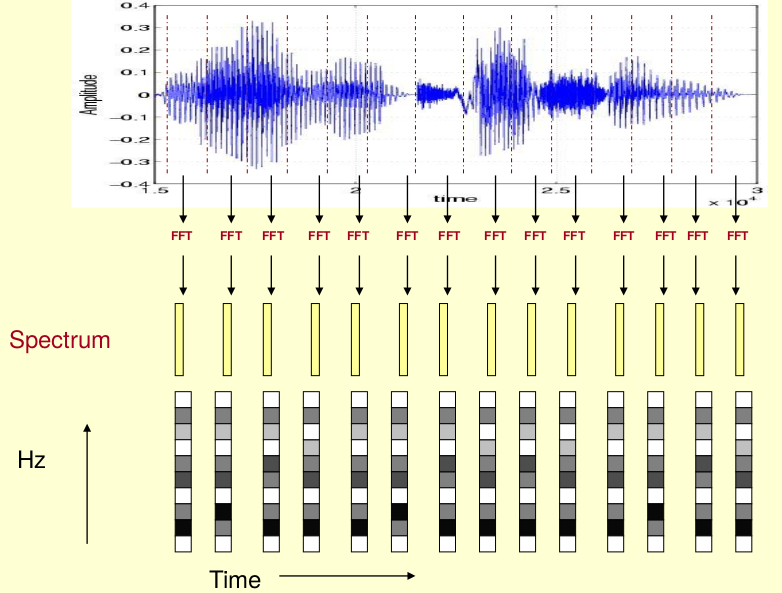
\includegraphics[height=5cm]{figure2.png}
    \caption{声码器获得频率分布}
\end{figure}
由于人耳对音高的敏感程度是指数的而不是线性的,频率一般会转换为梅尔标度(Mel scale,即 Melody Scale)\supercite{7}。梅尔标度并没有严格的定义,常用转换公式如下:
\begin{equation*}
    m=2595\log_{10}(1+\frac{f}{700})
\end{equation*}
在转换成频域后,声码器对其取频谱包络(Spectral Envelope)\supercite{8},即将不同频率的振幅最高点连线以得到一条平滑曲线。频谱包络曲线只需要对频谱曲线以频率为自变量做低通滤波即可。相当于利用低通滤波过滤掉快速变换的噪音,得到变换较慢的低频信号。除了求频谱包络以外,声码器还常使用梅尔滤波器组、梅尔倒谱系数(Mel-scaleFrequency Cepstral Coefficients,MFCC)和 DCT 离散余弦变换(DFT 离散傅里叶变换的简化版本)来求得音频的多维特征。

频谱包络描述了源 - 滤波器模型的滤波器部分,对频谱参数建模即可合成指定的音色和语素。CeVIO 和 Synthesizer V 等大部分现代语言合成引擎均采用此技术。

WORLD 是一个基于传统算法的开源声码器,WORLD 声码器将声音特征分为三部分:声音基频(F0),频谱包络(spectral envelop,sp)和非周期比值(aperiodicity,ap)。在源 - 滤波器模型中,F0 基频为源发出脉冲信号的频率,频谱包络 sp 为滤波器的频率响应。非周期比值 sp 则是语音中非周期信号的占比。前面提到过源除了能产生周期信号以外,还能产生白噪声来发气音。非周期信号占比指的就是白噪声占比。

在合成中,ap 与 sp 参数决定了歌声的音色和语素。因此只要调整 F0 和音素时长,就能够合成指定音色的歌声。WORLD声码器有开源python封装Pyworld,因此使用起来也比较方便。比如需要合成洛天依音源时,我们就可以使用山新的原声提取F0,并使用洛天依 v4 萌声库制作的无音高采样,用于提取包含音色和语素特征的 ap/sp 参数。\supercite{9}
\section{基于机器学习的声音合成}
基于数学建模的歌声合成逐渐遇到了瓶颈。数学建模的过程中对歌声机制做了很多简化(比如将人体的滤波器看做一个线性时不变系统),合成出的歌声细节不足,音质有时甚至不如波形拼接法。歌声合成的确是一个很适用机器学习算法的领域。人类歌声中频谱特性、音调、唱法多变,很难直接用数学建模。机器学习算法使用人类的歌声进行训练,识别其隐含的模式,并产生和人类类似的输出。
\subsection{机器学习乐谱处理}
利用机器学习进行声音合成的第一步是阅读乐谱以获得歌声的 F0 音高曲线,音素开始位置和音素时长。这些信息虽然可以直接由 midi 乐谱得到,但真实歌声要比乐谱复杂的多。歌手演唱时音与音之间会有滑音、转音,唱长音时有颤音,音的开始和结束处存在音高的微小波动。音素的开始位置和乐谱不同步,一般会不同程度的稍微提前。

在传统歌声合成软件中,软件根据 midi 乐谱生成大致的音高线,微调依赖用户手动完成。微调需要用户专门学习和训练,门槛相对较高。音素开始位置则内置于合成算法中,调整空间不大。
\subsection{机器学习生成频谱参数}
利用机器学习来获得声码器使用的频谱(共振峰)参数,相比传统建模分析更灵活,包括更多细节,例如高低音的音色区别,不同唱法的音色区别,咬字方式的动态变化,等等。以微软亚洲研究院的 XiaoiceSing(小冰歌声合成框架的早期版本)为例,在其论文中,框架的架构图如下:
\begin{figure}[H]
    \centering
    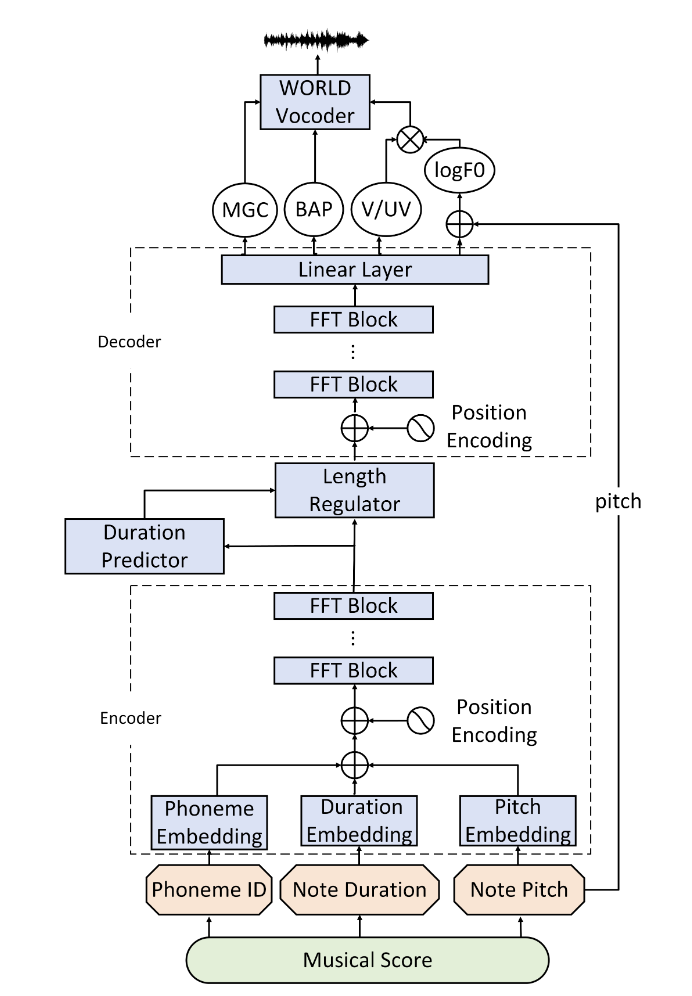
\includegraphics[height=10cm]{figure3.png}
    \caption{XiaoiceSing框架架构图}
\end{figure}
乐谱先转换成参数信息,再输入到由多个 FFT 块组成的编码器(Encoder)中。每个 FFT 块由一个 Self-Attention Network(SAN)和一个带有 ReLU 激活的两层 1-D 卷积神经网络(CNN)组成。编码器的输出会被一个一维 CNN 组成的音符时长预测器规范化。接下来,输出被送入由同样的 FFT 块构成的解码器(Decoder)以得到声音参数,即梅尔倒谱(mel-generalized cepstru,MGC)、非周期频段(band aperiodicit,BAP)、音高信息和清浊音(voiced/unvoiced,V/UV)标识。为了防止 AI 跑调,音高信息还要进行二次修正。

最后,XiaoiceSing 将生成的参数输入 WORLD 声码器以合成波形。其中 MGC 即为我们熟悉的 sp 谱,BAP 为 ap 谱,音高信息和清浊音标识结合得到 F0 参数。\supercite{10}
\subsection{机器学习声码器}
XiaoiceSing 由于算法自身不足和声码器的限制,所合成歌声的音质仍有提高空间。传统声码器正在逐步成为歌声合成系统的瓶颈。基于机器学习的声码器一般使用卷积神经网络(CNN)、生成对抗网络(GAN)等算法生成波形。代表有微软的 HifiSinger、谷歌的 Wavenet 等。这里以 RefineGAN 为例,以下为其项目架构图\supercite{11}:
\begin{figure}[H]
    \centering
    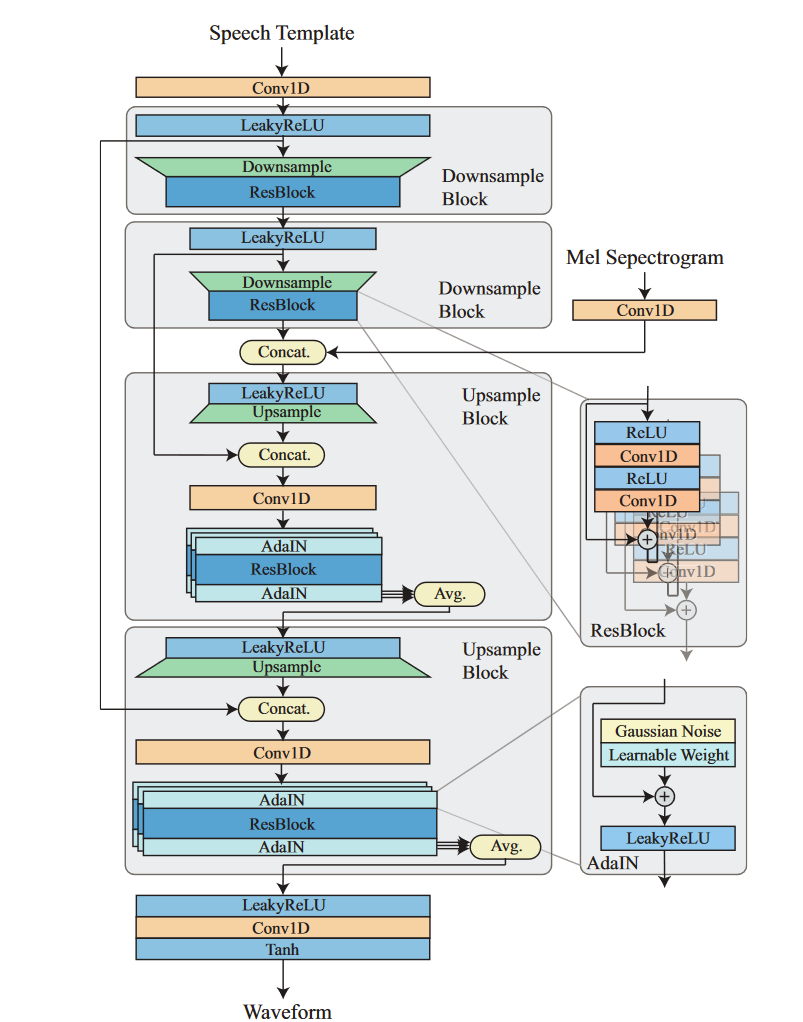
\includegraphics[height=12cm]{figure4.png}
    \caption{RefineGAN项目架构图}
\end{figure}
\section{总结}
在六十多年以前,刚刚让 IBM7904 唱响 Daisy Bell 的工程师们大概没有料到,歌声合成技术会在下一个世纪产生如此之大的影响力。从最简单的波形拼接法,再到利用数学建模方法研制出声码器进行歌声合成,直到现在随着机器学习的发展,我们可以用更多、更好的技术去实现歌声合成,并呈现出更多、更好的场面,无论是初音未来,还是洛天依、乐正绫,我们都能看到她们正在被越来越多的人喜爱着,并希望贡献自己的力量以帮助实现更好的她们。

\newpage
\small

\begin{thebibliography}{99}
    \setlength{\parskip}{0pt}

    \bibitem{1} "The Sounds of Fighting Men, Howlin' Wolf and Comedy Icon Among 25 Named to the National Recording Registry". Loc.gov. Retrieved 8 January 2021.
    \bibitem{2} 《流浪地球 2》李雪健人类股骨演讲发布,消息称采用 AI 修复声音.
    https://www.ithome.com/0/668/218.htm
    \bibitem{3} Wolfe, Joe et al. “An Experimentally Measured Source–Filter Model: Glottal Flow, Vocal Tract Gain and Output Sound from a Physical Model.” Acoustics Australia 44 (2016): 187-191.
    \bibitem{4} 语音信号处理-语音产生模型 https://zhuanlan.zhihu.com/p/499181697
    \bibitem{5} Wikipedia.Vocaloid\_6: https://zh.wikipedia.org/wiki/Vocaloid\_6
    \bibitem{6} Cepstrum Analysis, Mel-Frequenantkillerfarm.github.io/speech/2018/06/06/speech\_5.html\#mel-frequency-analysis
    \bibitem{7} WikiPedia.Mel\_Scale: https://en.wikipedia.org/wiki/Mel\_scale
    \bibitem{8} Siedenburg, K., Jacobsen, S., \& Reuter, C. (2021). Spectral envelope position and shape in sustained musical instrument sounds. Journal of the Acoustical Society of America, 149(6), 3715–3726. https://doi.org/10.1121/10.0005088
    \bibitem{9} WORLD vocodor: https://github.com/mmorise/World
    \bibitem{10} Lu, Peiling et al. “XiaoiceSing: A High-Quality and Integrated Singing Voice Synthesis System.” Microsoft Research Asia. https://doi.org/10.48550/arXiv.2006.06261
    \bibitem{11} Xu, Shengyuan et al. “RefineGAN: Universally Generating Waveform Better than Ground Truth
    with Highly Accurate Pitch and Intensity Responses” timedomain. Inc https://doi.org/10.48550/arXiv.2111.00962





\end{thebibliography}
\end{document}